\documentclass{ximeraXloud}

\title{French History and Dinosaurs!}
\begin{document}
\begin{abstract}
    This section introduces the origin an application of graphing.
\end{abstract}
\maketitle

Yes, history in a math class, but this helps demonstrate both how natural the Cartesian graphing system is, and where it came from... not to mention who invented it. 

As the (possibly apocryphal) story goes, Rene Descarte, a famous seventeenth century philosopher%
\footnote{
    He was the one who famously said ``cogito ergo sum" ie ``I think, therefore I am."
    }%
and mathematician, was sitting in bed one day with a cold and watching a fly crawling across his ceiling. He started trying to figure out how he'd describe the fly's path to a friend later when he realized that it would be easiest to just record the fly's distance from two adjacent walls of his room at each time of interest. By saying the fly was `3 inches from the south wall and 4 inches from the east wall' one could \textit{precisely} state the location of that fly at that moment, even if the fly was no longer present. Thus he came up with the idea of the coordinate axis system, the `x-y plane'. We even named this plane after him; the so-called ``Cartesian Plane''. 

\subsection*{Uses for the Cartesian plane and graphing}
    Graphing on the Cartesian plane has two (very) distinct uses. We will introduce the most commonly used form (outside of academics) of Cartesian graphing here, but for the rest of this class (and calculus one) we will only utilize the second usage, which we cover in the next tile on how to graph to relate variables.

    \subsubsection*{Grid system and Dinosaurs!}
        The first way that Cartesian graphing is commonly used is as a coordinate system to allow one to be precise about the location of something that is found within a larger context. A great example of this is when archaeological dig sites are documented. A (properly) documented archaeology site will superimpose a grid over the entire site, where one axis will be assigned numbers and the other axis will be assigned letters. Thus you might have a grid where the East/West direction is labeled with ``A'' at end and assigning a letter to each block across the axis. Similarly the North/South most section could be labeled with a ``1'' at one end, and labeling with progressively larger numbers along the axis for each subsequent block. You would end up with something like Figure \ref{gridMap}
        
        \begin{figure}[h]
            \begin{center}
                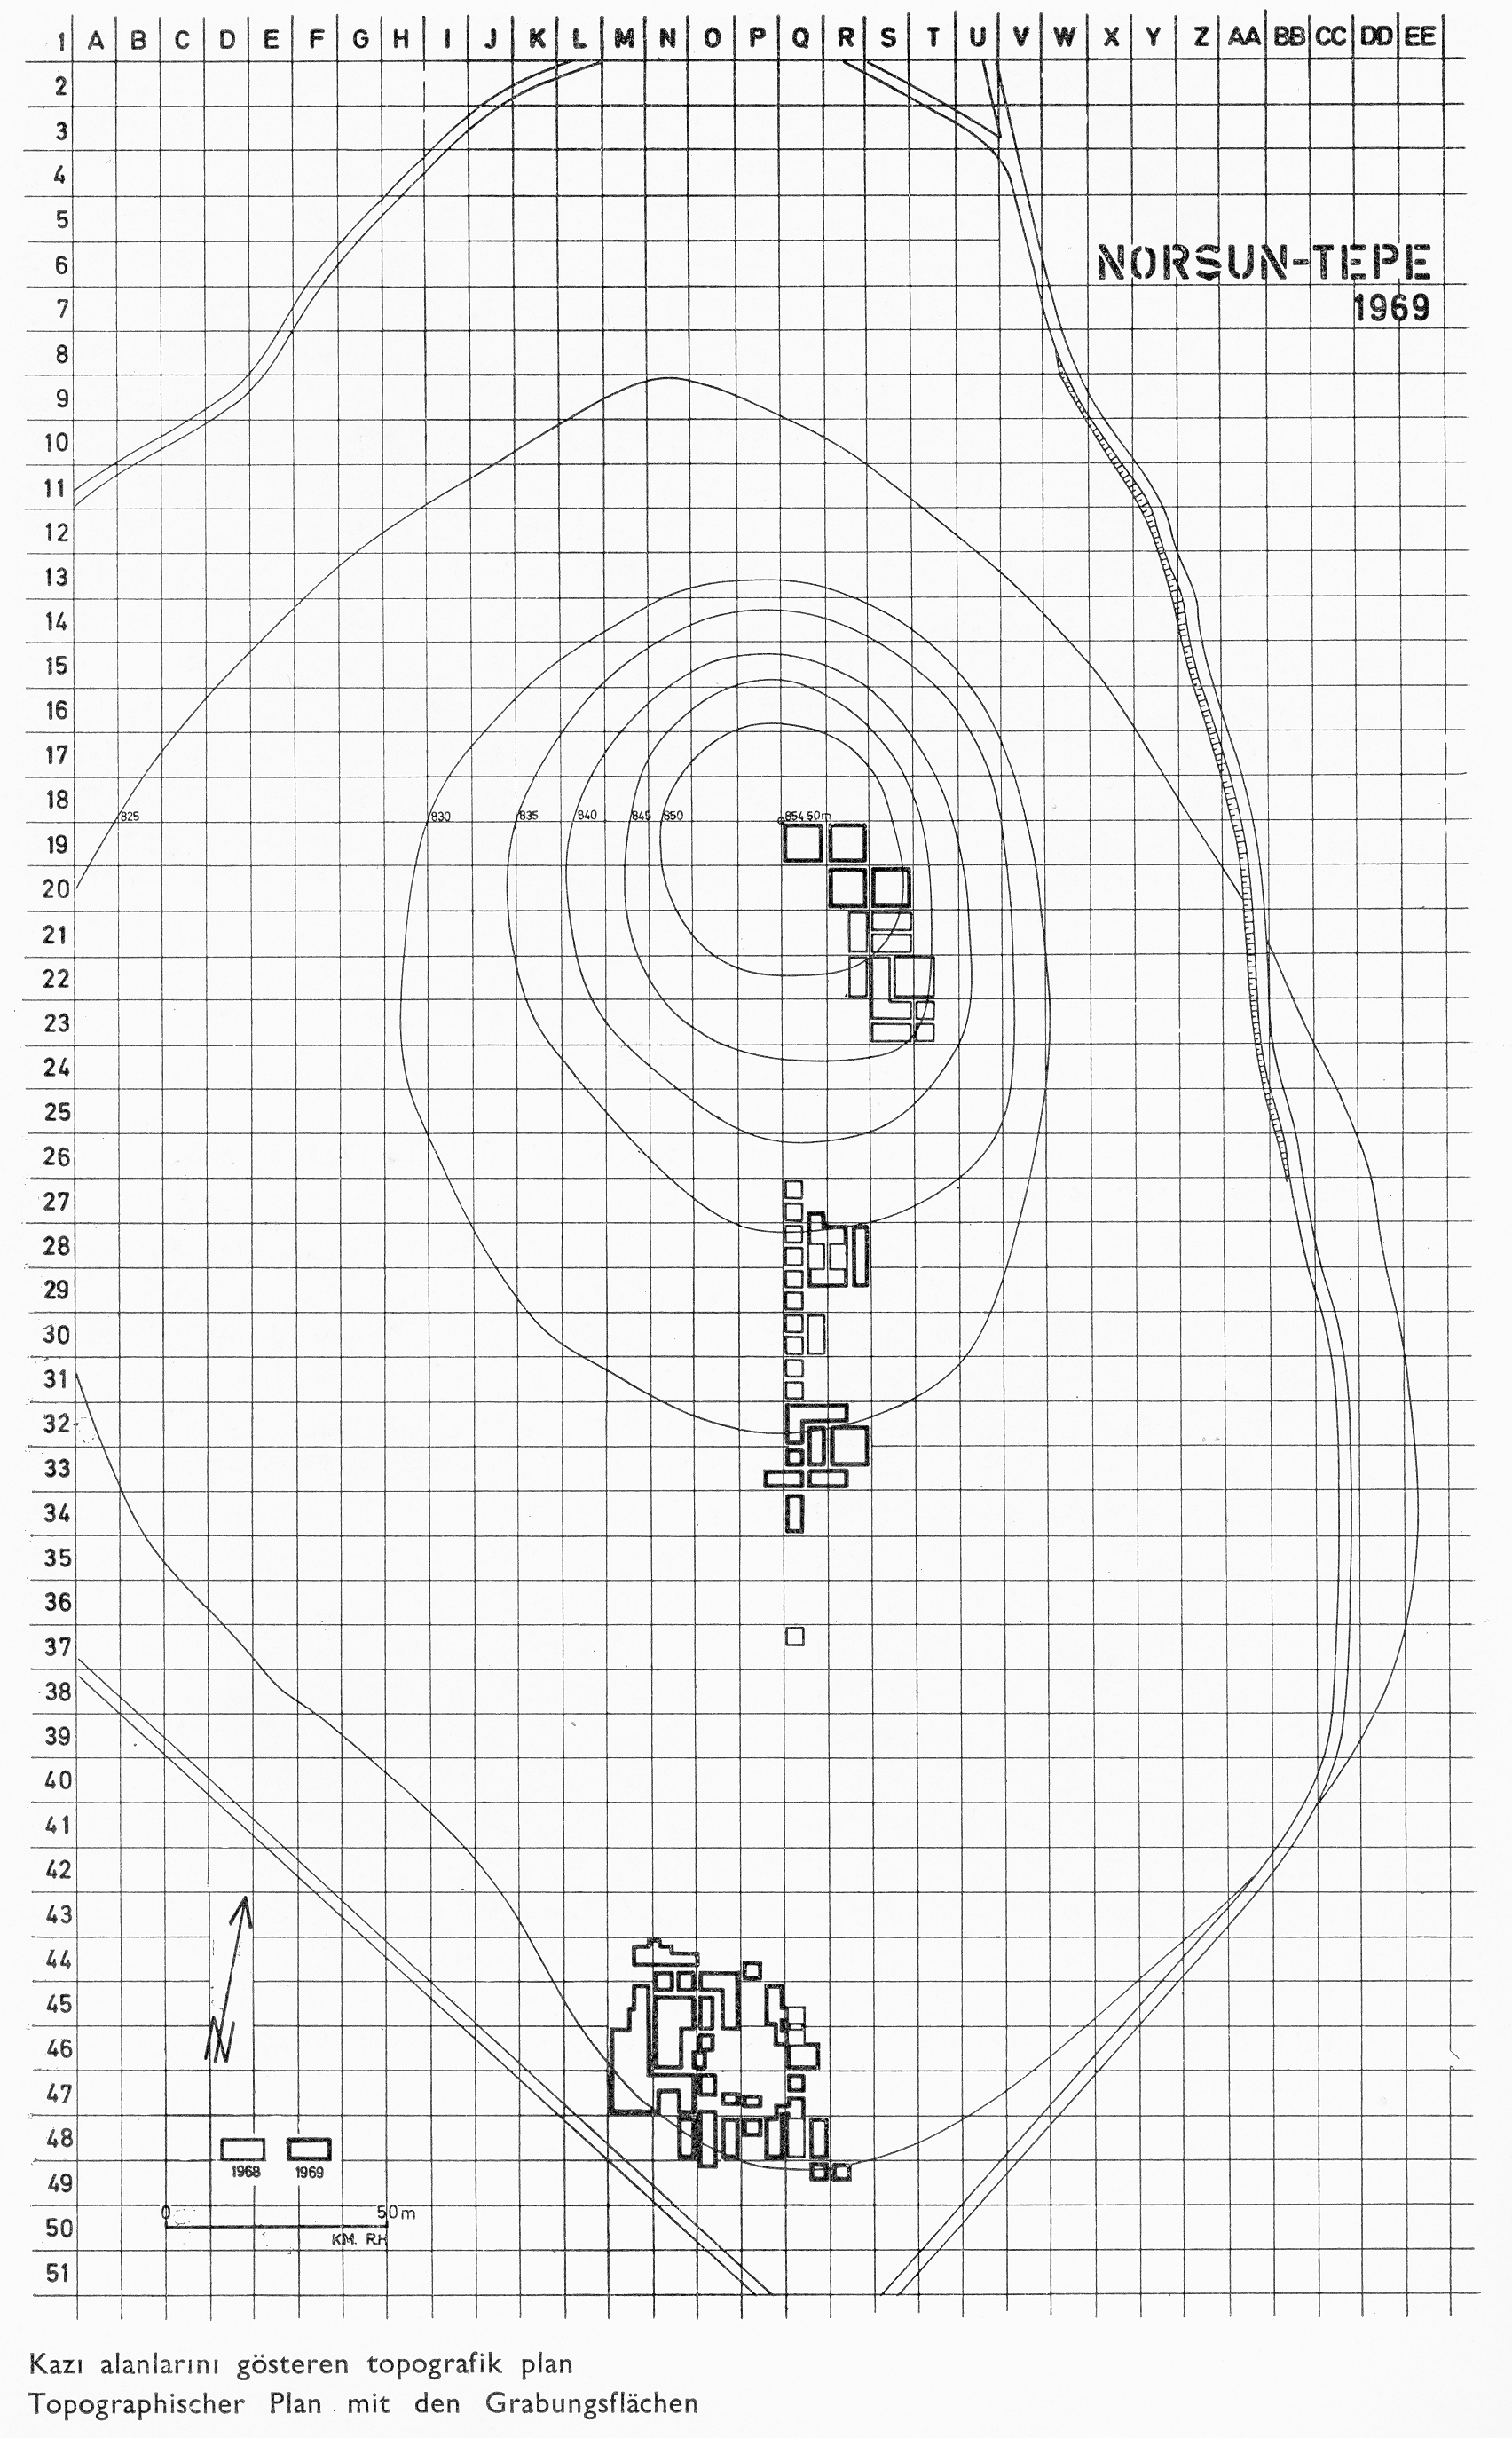
\includegraphics[scale=0.5]{/home/jason/Dropbox/Teaching/MAC1140/xronosTextXloud/graphing/archeologyGrid.jpg}
            \end{center}
            \caption{
                An actual archaeological digsite map of a religious site in Turkey, originally drawn in 1963 and reprinted in 1969. Actual research and corresponding archaeological digs didn't begin until 1995.
                }
            \label{gridMap}
        \end{figure}
        
    \begin{problem}
        So, who do we have to blame for learning graphing in the plane?
        \begin{multipleChoice}
            \choice{Math teachers. They are clearly sadists.}
            \choice{Whomever wrote the curriculum for this class.}
            \choice[correct]{Rene Descarte; and the stupid fly on his wall.}
            \choice{I blame nobody. Or everybody. Definitely everybody.}
        \end{multipleChoice}
    \end{problem}
    
    \begin{problem}
        What type of graphing would most commonly be used by archaeologists or landscapers?
        \begin{multipleChoice}
            \choice[correct]{Determining where major features are and/or as a way of sectioning off land for further work or study.}
            \choice{A way to differentiate who is going to work where to determine payment.}
            \choice{Determining the age of the land in order to setup a heirarchy for what to work on first.}
            \choice{They don't use graphing.}
        \end{multipleChoice}
    \end{problem}

\end{document}